\chapter{Appendix}

\begin{table}
\centering
\caption{Line fidelity as a function of S/N and line width.}
\begin{tabular}{cccccccccc}
\hline
S/N & 3 chn & 5 chn & 7 chn & 9 chn & 11 chn & 13 chn & 15 chn & 17 chn & 19 chn \\
\hline
5.85 & 0.09 & 0.07 & 0.15 & 0.12 & 0.11 & 0.1 & 0.17 & 0.14 & 0.26 \\
5.95 & 0.15 & 0.14 & 0.3 & 0.23 & 0.24 & 0.2 & 0.31 & 0.23 & 0.48 \\
6.05 & 0.26 & 0.27 & 0.51 & 0.41 & 0.44 & 0.36 & 0.51 & 0.37 & 0.72 \\
6.15 & 0.4 & 0.45 & 0.71 & 0.62 & 0.67 & 0.56 & 0.7 & 0.54 & 0.87 \\
6.25 & 0.56 & 0.66 & 0.86 & 0.79 & 0.84 & 0.75 & 0.85 & 0.7 & 0.95 \\
6.35 & 0.71 & 0.82 & 0.94 & 0.9 & 0.93 & 0.87 & 0.93 & 0.82 & 0.98 \\
6.45 & 0.83 & 0.91 & 0.97 & 0.96 & 0.97 & 0.94 & 0.97 & 0.9 & 0.99 \\
6.55 & 0.91 & 0.96 & 0.99 & 0.98 & 0.99 & 0.97 & 0.99 & 0.95 & 1.0 \\
6.65 & 0.95 & 0.98 & 1.0 & 0.99 & 1.0 & 0.99 & 0.99 & 0.98 & 1.0 \\
6.75 & 0.98 & 0.99 & 1.0 & 1.0 & 1.0 & 1.0 & 1.0 & 0.99 & 1.0 \\
6.85 & 0.99 & 1.0 & 1.0 & 1.0 & 1.0 & 1.0 & 1.0 & 0.99 & 1.0 \\
6.95 & 0.99 & 1.0 & 1.0 & 1.0 & 1.0 & 1.0 & 1.0 & 1.0 & 1.0 \\
7.05 & 1.0 & 1.0 & 1.0 & 1.0 & 1.0 & 1.0 & 1.0 & 1.0 & 1.0 \\
7.15 & 1.0 & 1.0 & 1.0 & 1.0 & 1.0 & 1.0 & 1.0 & 1.0 & 1.0 \\
7.25 & 1.0 & 1.0 & 1.0 & 1.0 & 1.0 & 1.0 & 1.0 & 1.0 & 1.0 \\
7.35 & 1.0 & 1.0 & 1.0 & 1.0 & 1.0 & 1.0 & 1.0 & 1.0 & 1.0 \\
7.45 & 1.0 & 1.0 & 1.0 & 1.0 & 1.0 & 1.0 & 1.0 & 1.0 & 1.0 \\
7.55 & 1.0 & 1.0 & 1.0 & 1.0 & 1.0 & 1.0 & 1.0 & 1.0 & 1.0 \\
7.65 & 1.0 & 1.0 & 1.0 & 1.0 & 1.0 & 1.0 & 1.0 & 1.0 & 1.0 \\
7.75 & 1.0 & 1.0 & 1.0 & 1.0 & 1.0 & 1.0 & 1.0 & 1.0 & 1.0 \\
7.85 & 1.0 & 1.0 & 1.0 & 1.0 & 1.0 & 1.0 & 1.0 & 1.0 & 1.0 \\
7.95 & 1.0 & 1.0 & 1.0 & 1.0 & 1.0 & 1.0 & 1.0 & 1.0 & 1.0 \\
\end{tabular}
\end{table}\label{table:Fid_Table}

\section{Line Candidates}\label{sec:A1}

The following plots show the 35 CO line candidates in various wavelengths. The red contours show the  +2$\sigma$,4$\sigma$,6$\sigma$,and 8$\sigma$ values in the datacubes. 

\begin{figure}[tbp]
\centering 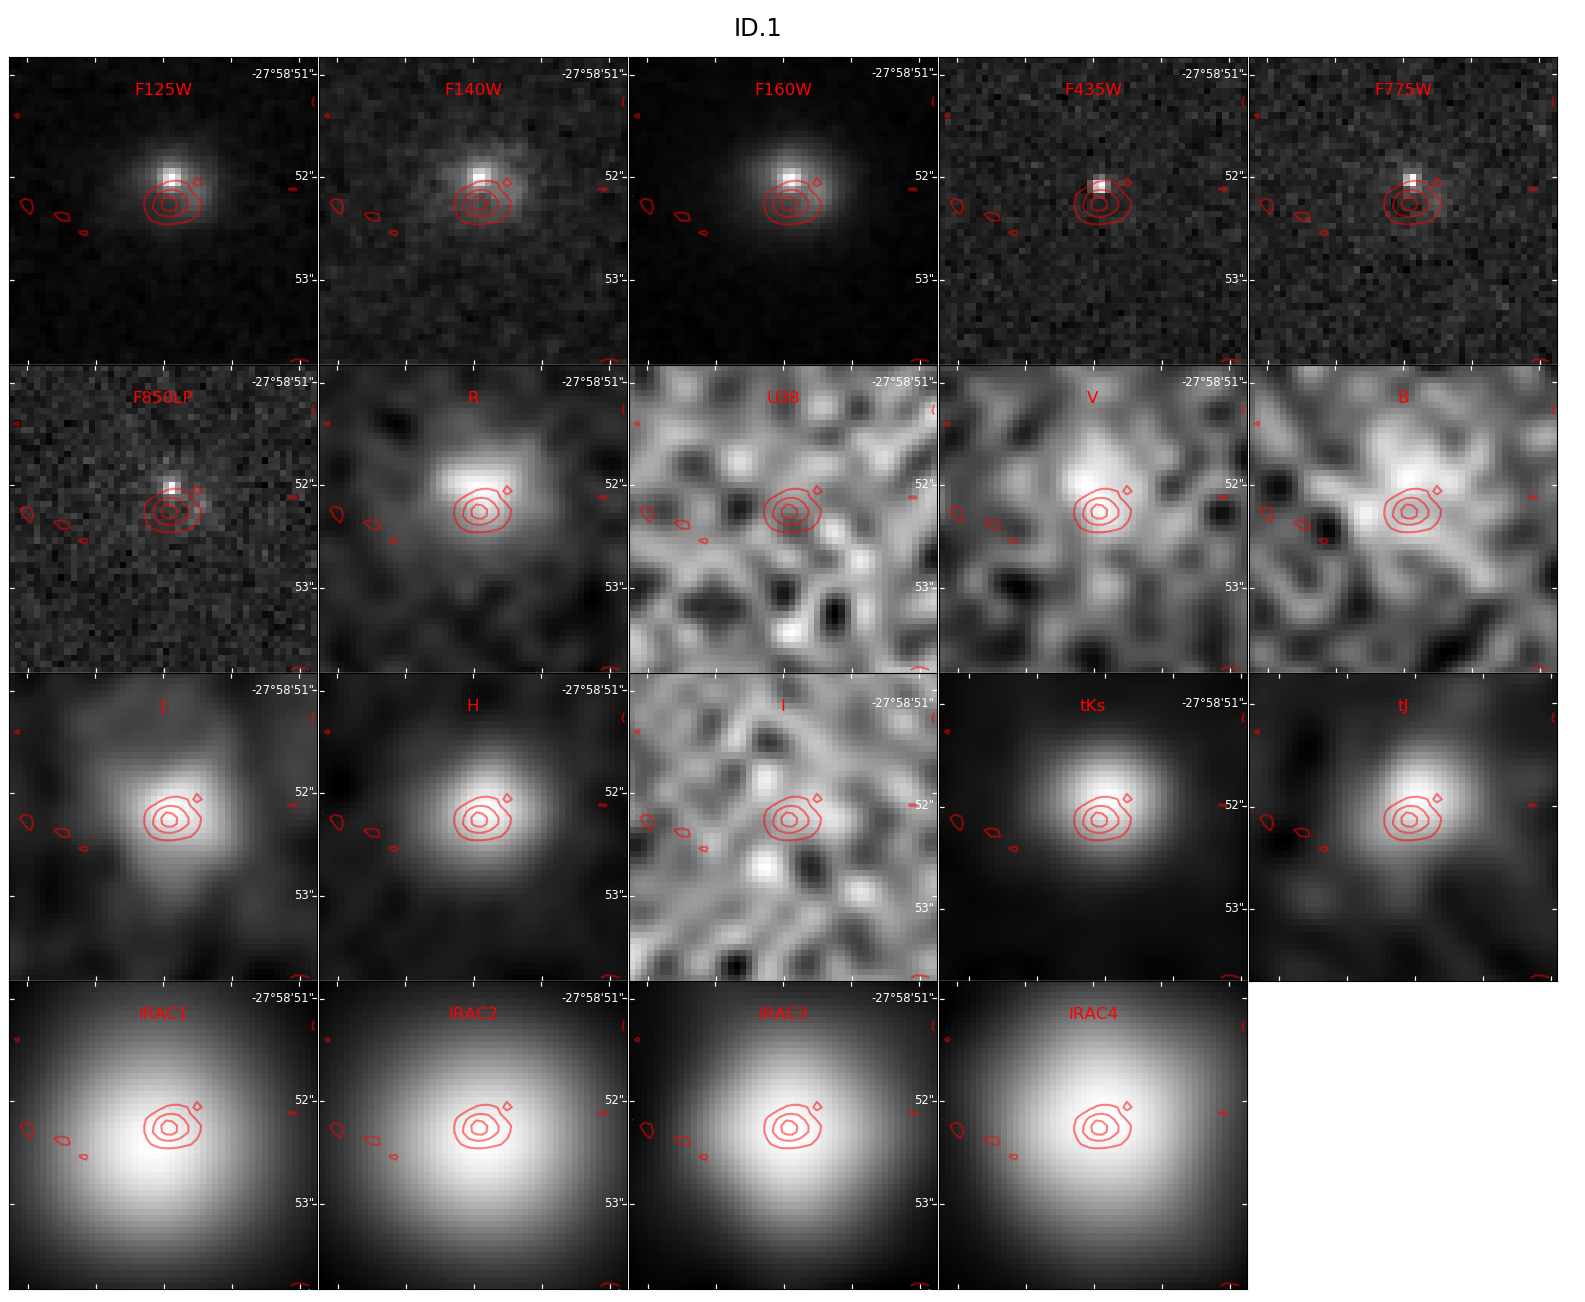
\includegraphics[width=120mm]{Matched/ASPECS_Cutout_0.jpg}
\caption{ID.1}
\label{fig:Match_One}
\end{figure}

\begin{figure}[tbp]
\centering 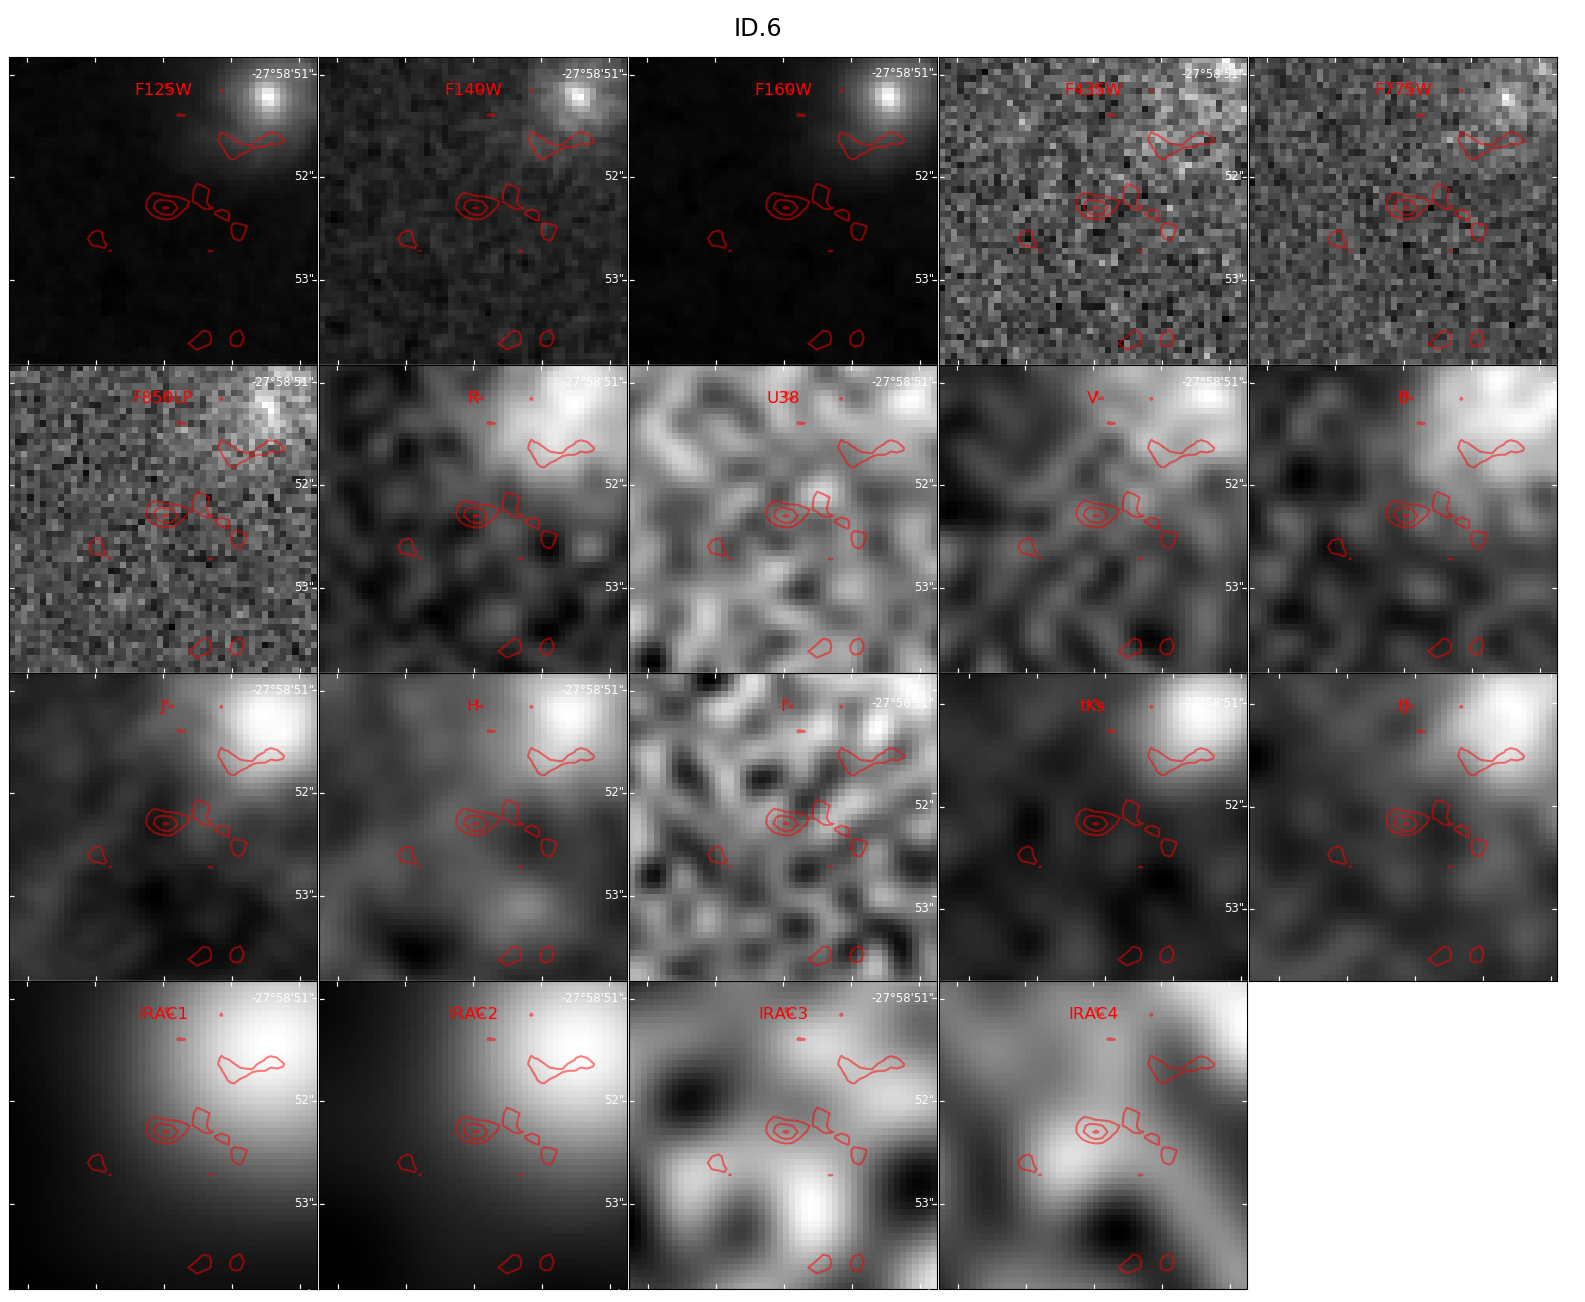
\includegraphics[width=120mm]{Matched/ASPECS_Cutout_5.jpg}
\caption{ID.5}
\label{fig:Match_Three}
\end{figure}


\begin{figure}[tbp]
\centering 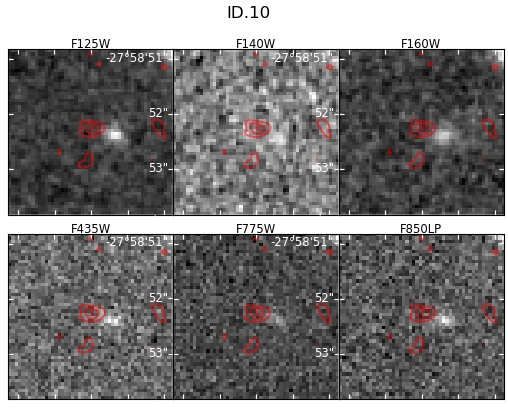
\includegraphics[width=120mm]{Matched/ASPECS_Cutout_9.jpg}
\caption{ID.9}
\label{fig:Match_Three}
\end{figure}


